\documentclass[a4paper,11pt,fleqn, titlepage]{article}

\usepackage[utf8]{inputenc}
\usepackage[swedish]{babel}
\usepackage[lighttt]{lmodern}
\usepackage{parskip}
\usepackage{amsmath}
\usepackage{amssymb}
\usepackage{amsthm}
\usepackage{listings}
\usepackage{graphicx}
\usepackage{biblatex}
\usepackage{csquotes}


\addbibresource{referenser.bib}

\author{Andreas Hagesjö \and Daniel Pettersson \and
Magnus Hagmar \and Niclas Ogeryd \and Robert Nyquist}

\title{Fossilfri bilflotta \\ Kurs ENM155}


\begin{document}
\maketitle

\section{Introduktion}
I denna rapport undersöks möjligheterna för att göra Sveriges bilflotta
fossiloberoende till år 2030. Just nu kommer den största delen av energin
som används i transportsektorn från just fossila bränslen. Detta betyder
såklart att väldigt mycket utsläpp orsakas av alla bilar, utöver den stora
energiförlusten på grund av den låga verkningsgraden för
förbränningsmotorer. Genom att bryta beroendet utav fossila bränslen
förbättras miljön alltså både genom minskade utsläpp och energiförbrukning.

Denna frågeställning är intressant att studera eftersom regeringen har satt
just detta mål för Sverige. Utöver detta så är det både ett aktuellt ämne
i samhället samt att det enligt flera utförda studier går att uppfylla
målsättningen. Denna rapport innehåller en modell som visar vilka energier
som kan användas för att nå detta mål samt olika scenarier för hur målet
kan uppnås. För att det skall vara möjligt så krävs det vissa
ansträngningar och tekniska utvecklingar.

Vad fossiloberoende betyder kan vara en tolkningsfråga, men i denna rapport
används det med betydelsen att det är \emph{möjligt} för bilflottan att
köras på fossilfria bränslen, men att det inte måste vara så. Att ha tillgång
till fossila bränslen och möjlighet att använda det kan vara viktigt för
att upprätthålla bränslesäkerhet ifall det blir en temporär brist på
några av alternativen.

\subsection{El}

För personbilar så kommer eldrift att ersätta stor del av bensin- och
dieseldrift. Då elbilar är effektivare än bilar med förbränningsmotorer så
kommer bytet till elbilar medföra att mängden energi som behöves för att
driva bilflottan att minska \cite[s.~25]{elforsk}. Då stor del utav
elbilarna som säljs idag är laddhybrider, Mitsubishi Outlander står ensam
för nästan 30 procent av det laddbara beståndet i Sverige, så kommer den
typen av bilar fortfarande rulla 2030 och därmed fortfarande använda
fossilt bränsle \cite{laddbarafordon}. I nuläget så är det endast
7800 av de cirka 4.5 miljoner bilarna i Sverige som kan drivas på
el \cite{fordonsstatistik}.\\

Det kommer att diskuteras huruvida
utvecklingen kan ske till 2030 för att se till att eldrivna bilar kommer
att bli en mer betydande del av fordonsflottan gentemot hur det ser ut
idag, och att efterfrågan för elbilarna kommer att öka drastiskt.
Regeringen har i nuläget infört styrmedel för att gynna elbilar
(och de absolut bästa gasbilarna), med en supermiljöbilspremie, som innebär
att om en bils maximala koldioxidsläpp per kilometer är 50 gram, så kan denna
premie tilldelas \cite{ekonomiskastyrmedel}.\\

En fråga man kan ställa sig är huruvida det kommer gå att producera den
extra mängden el som behöves för att utöka beståndet med elbilar. Som det
ser ut nu så skulle bilflottan behöva runt 53 TWh/år år 2030 utan några
åtgärder \cite[s.~24]{elforsk}, men med
den effektiviseringen som kommer med elmotorer, mellan 2,5 och 3 gånger så
effektiv \cite[s.~29]{elforsk}, så kommer den
mängden energi att minska så pass mycket att det inte blir nödvändigt med
så stor ökning utav elproduktionen.

\subsection{Biobränsle}
Tunga fordon så som lastbilar och maskiner kommer antagligen inte kunna
köras med eldrivna motorer inom de nästkommande åren, detta på grund av att
man idag inte kan lagra den mängden energi som behövs för att driva ett
stort och tungt fordon. Och eftersom de flesta tunga fordon idag körs på
diesel, kan ett bränslebyte till biodiesel gå relativt smärtfritt.

Samma sak är det med bensin och dieselbilar som säljs idag, eftersom
medelåldern på en personbil i Sverige är 9 år \cite[s.~17]{elforsk} så
betyder det att det kommer köras bilar år 2030 som är sålda idag,
och då måste vi ha ett sätt att med så låg kostnad som möjligt, konvertera
dessa till fossilfria alternativ. Där ligger biobränslen närmast; en bil
som idag körs på diesel kan, som tidigare sagt, relativt smärtfritt köras
på biodiesel istället \cite{statoil}. Lite
svårare bil det däremot med en bensindriven bil. Där kan man bli tvungen
att göra lite större ändringar i motorn vilket självklart resulterar i en
högre kostnad för konverteringen. Denna konvertering är mycket möjligt att genomföra.
Detta betyder att bilar som säljs idag och några år framåt,
som är avsedda att köras fossila bränslen som bensin och diesel, kan
konverteras och då framföras oberoende av fossila bränslen.

För att främja biobränslet i Sverige har man i nuläget infört ekonomiska styrmedel
genom att låta allt biobränsle genom att låta dess skatt vara
avdragsgill \cite{ekonomiskastyrmedel}.

Man får dock vara försiktig med just biobränslen; det finns inte
biobränslen i överflöd. Skulle andra länder få en ökad efterfrågan på
biobränslen kan det få priset att rusa i taket. Detta kan medföra stora
negativa effekter så som \emph{land-grabbing} \cite{bioenergi}, ökade matpriser i
fattigare länder etc. vilket man då kan reglera genom att man har kvar
möjligheten att tillfälligt köra på fossila bränslen, för att minska
Sveriges efterfrågan på biobränslen dels ur bränslesäkerhet men även
miljömässigt och kanske även ur ett etiskt perspektiv.

\subsection{Vätgas}
Bilar som drivs på vätgas ligger för tillfället bakom både elbilar och
bilar som drivs på biobränsle. Därför räknar vi med att år 2030 så
består inte stora delar utav bilflottan av bilar som drivs av vätgas.
Bilarna produceras fortfarande i små mängder och i Sverige finns endast en
laddningsstation för tillfället \cite{macken}.
Bilarna är dessutom fortfarande för dyra för att få ett stort genomslag än så länge. Bilar som drivs på vätgas har har stor potential i framtiden men 2030 så kommer de inte finnas i lika stor mängd som elbilar och biobränslebilar.

\subsection{Kärnkraft}
Regerigen har upphävt förbudet mot ny kärnkraft i Sverige. Detta har lett till intresse till ersätta gamla reaktorer med nya, bland annat i Oskarshamn, som kan producera mer el.
Dessutom så kan man räkna med att samtliga aktiva reaktorer i Sverige
kommer att producera en större mängd el om 15 år än vad de gör nu
\cite[s.~80]{karnkraft}. Därför räknar vi med att kärnkraften år 2030 har möjlighet att täcka upp för det ökade behovet utav elproduktion som en ökad mängd elbilar medför.

\section{Metod}
Vi har utgått från den angivna modellen i tidigare uppgift. Med den som
ursprungsläge samt information från flera rapporter och prognoser i ämnet
har vi kunnat få fram en hypotes till hur energisystemet kan komma att se
ut 2030. Vi har sedan matat vår algoritm med hypotesen. Den har sedan räknat ut
resultatet och visar det i den form som vi behöver.

\begin{figure}[h!]
	\centering
	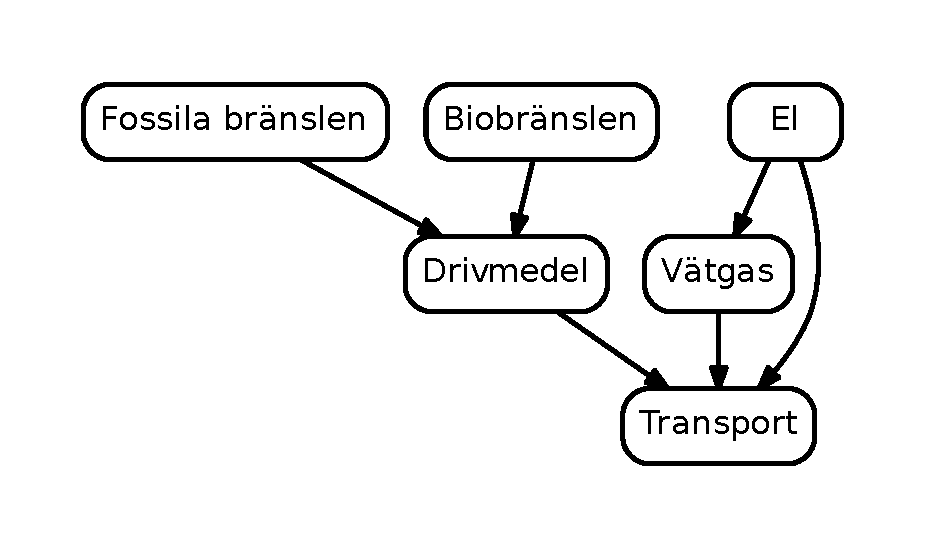
\includegraphics[scale=0.70]{diagram.pdf}
	\label{modell}
	\caption{Förenklad modell av transportsektion.}
\end{figure}

Den nuvarande modellen över transportsektorn ser förenklad ut som i figur
\ref{modell}. På pilarna mellan lådorna ska det såklart vara
transmissionsförluster och verkningsgrader, men eftersom dessa varierar i
de olika scenarierna har vi valt att inte skriva ut dessa.

Fördelen med vårt tillvägagångssätt är att vi kan vara säkra på att vårt
resultat är korrekt beräknat då vi har matematiken att falla tillbaka på.
Så resultatet från vår algoritm är korrekt. En nackdel är dock att vi inte
kan vara säkra på att vår indata till algoritmen är korrekt då det är
omöjligt för oss att säga hur verkligheten kommer att se ut 2030. Hypotesen
vi har är så realistisk som vi kunde få den till med hjälp av den datan som
vi kommit över. Vi har inte räknat med några stora oförutsedda scenarion,
utan mer eller mindre räknat med att övriga områden ska fortsätta utvecklas
som vanligt.


\section{Resultat}

\subsection{Scenario 1 - Biobränslen och elbilar}

För att ersätta fossila bränslen så är som bekant de två huvudalternativen
biobränslen eller elbilar. I detta scenario så utvecklas både användningen
av biobränslen, samtidigt som en del av bilflottan byts ut mot el- eller
hybridbilar.

Enligt Regeringens utredning 2013 så kan energianvändningen hos
förbränningsmotorer för personbilar väntas minska med ca 28 procent till år
2030 \cite{fossilfrihet}. Denna utveckling gör att verkningsgraden utav
drivmedel ökar med åtta procentenheter från 20 till 28\%.  Totalt sett så
kan energianvändningen för personbilar väntas minska med 43-50\% om elbilar
och laddhybrider vid eldrift står för drygt 40 procent av körsträckan
\cite{fossilfrihet}.  Energianvändningen minskar dock inte såhär mycket 
eftersom verkningsgraden för att framställa drivmedel utav biomaterial
är 45\% lägre än för fossila bränslen.

Bilar som drivs helt eller delvis med el förväntas göra så att el står för
någonstans mellan 3 och 14 procent av den totala energianvändningen hos
vägtrafiken.

Energianvändningen för tunga fordon, sjöfart, bantrafik samt flyg förväntas
minska något också, då man tror att de kommer ha en effektivisering på 10-14 procent.
Just nu står vägtrafiken för 94\% av hela sektorns förbrukade energi\cite[s.~11]{el2013}, och
om de olika trafikslagen upptar lika stor andel av transportsektorns
förbrukning år 2030 som nu så kommer energianvändningen se ut som i tabell
\ref{tab:scen1energi}. Fördelningen av energislag visas även i figur \ref{fig:scen1energifordelning}.

\begin{figure}[h!]
       \centering
       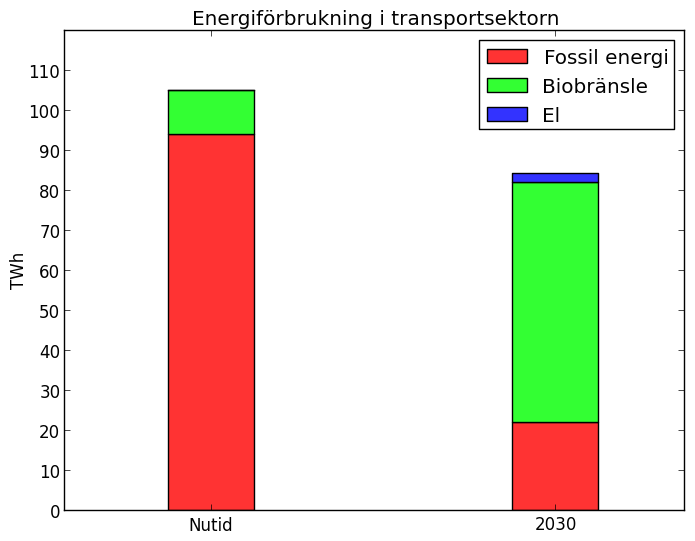
\includegraphics[scale=0.7]{scen1a1transport.png}
       \caption{Fördelning av energi i transportsektorn nu och år 2030}
       \label{fig:scen1energifordelning}
\end{figure}

\begin{figure}[h!]
	\begin{center}
	\begin{tabular}{ | l | l | l | }
	\hline
						& Nu		& 2030 \\ \hline
	Fossil energi				& 94 TWh	& 22,2 TWh \\ \hline
	Biobränsle				& 11 TWh	& 60 TWh \\ \hline % 91% av energianvändningen
	El					& (Nästan) 0 TWh &  2,2 TWh \\ \hline % ~6% av bilenergianvändningen
	Total energianvändning		& 105 TWh	& 86 TWh \\ \hline
	Energianvändning av personbilar	& 50 TWh	& 35 TWh \\ \hline
	\end{tabular}
	\caption{Energianvändning i transportsektorn}
	\label{tab:scen1energi}
\end{center}
\end{figure}

Som man kan se så kommer fossila energikällor stå för knappt en fjärdedel så mycket energi år 2030. Den kvarvarande fossila energin används av tunga fordon och andra transporter än vagtrafik. Bioenergi står för den överlägset största delen av energitillförseln, och några sätt att nå upp till denna nivå presenteras i sektion \ref{subsec:scen1}.

\subsection{Vätgas-scenario}
En form av elbilar som i framtiden kan tänkas få en större utbreddning är
bränslecellsbilar (FCEV - Fuel Cell Electric Vehicle). I dessa används en
bränslecell, förslagsvis driven på vätgas, för att generera el som sedan
driver en elmotor. Här finns även möjligheten att låta bränslecellen ladda
ett batteri, en s.k. bränslecellsladdhybrid. En fördel med bränsleceller
över traditionella elbilar är längre körsträckor (ca 500km)
\cite{fossilfrihet}. Den stora nackdelen med bränslecellsfordon är den höga
kostnaden som i dagens läge ligger på ca 50\$/kWh \cite{fossilfrihet}.

Verkningsgrader
Elektrolys vid tankstationer

El för att ladda ett batteri ger ca 83\% verkningsgrad, om samma mängd används för vätgas genom elektrolys - 34\%

En stor fördel med FCEV är räckvidden, som är betydligt högre än hos
elbilar. Detta gör den till ett attraktivt alternativ när det gäller
fordorn fria från koldioxidutsläpp. Kostnaden för FCEV samt tillhörande
bränsle räknas även att minska med ca 90\% fram till 2020 \cite{mckinsey}.

\footnote{Källa: regeringsrapport och mckinsey-rapport}.
(20\% FCEVs, 20\% BEVs, 25\% PHEVs and 35\% ICEs).

Indata - baserat på
bränsle 55\% 0.55*35 = 8.8
elbil 25\% 0.25*35 = 4
väte 20\% amount = 0.2*35 = 3.2

Verkningsgrad FCEV 34\%
Verkningsgrad BEV 83\%
Verkningsgrad PHEV ungefär samma som BEV 83\%
Verkningsgrad ICE 28\%

\begin{figure}[h!]
       \centering
       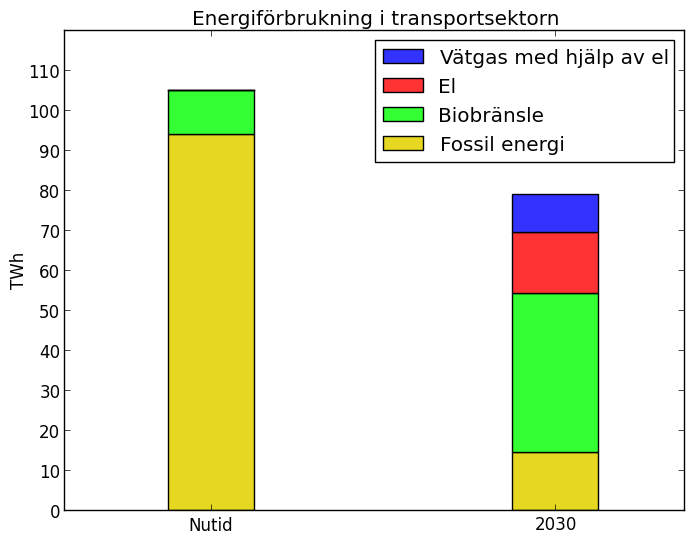
\includegraphics[scale=0.7]{scen2transport.png}
       \caption{Awesome Imagelol}
       \label{fig:scen2transport}
\end{figure}

SKRIV SKIT HÄR

\begin{figure}[h!]
	\centering
	\label{tab:scen2energi}
	\begin{tabular}{ | l | l | l | }
	\hline
						& Nu		& 2030 \\ \hline
	Fossil energi				& 94 TWh	& 14.7 TWh \\ \hline
	Biobränsle				& 11 TWh	& 39.7 TWh \\ \hline % 91% av energianvändningen
	El					& (Nästan) 0 TWh &  15.3 TWh \\ \hline % ~6% av bilenergianvändningen
	|- varav Vätgas     & (Nästan) 0 TWh & 9.4 TWh\\ \hline
	Total energianvändning		& 105 TWh	& 79.9 TWh \\ \hline
	Energianvändning av personbilar	& 50 TWh	& 32.5 TWh \\ \hline
	\end{tabular}
\end{figure}

NÄMEN LITE MER SKIT HÄR

\section{Diskussion}

\subsection{Scenario 1}
\label{subsec:scen1}
Scenario 1 är möjligt att genomföra på flera olika sätt och här kommer det diskuteras två olika lösningar. 
Det finns vissa gemensamma problem och åtagande för båda lösningarna.

Ökad användning utav biobränsle är ett måste. Detta behöver man vara väldigt försiktig med i början, då ökad produktion måste göras i kontrollerade mängder så det inte leder till höjda markpriser vilket kan bidra till ökad pris på mat och land-grabbing.
Enligt regeringens rapport så kommer Sverige att kunna producera 50-60 TWh mer biomassa per år, vilket motsvarar 25-30 TWh mer biodrivmedel jämfört med dagens mängd. Detta kommer förmodligen inte att vara tillräckligt för att täcka det behovet som en stor utökning utav bilar som drivs på biodrivmedel orsakar, alltså kan Sverige komma att behöva importera biomassa från anda länder.

Mängden el som kommer användas samt behöva produceras ändras med dessa genomföranden och detta är möjligt att göra på olika sätt, vilket diskuteras i de olika alternativen.

Det är inte bara mängden energi och fördelningen som måste lösas utan man måste även övertyga Sveriges bilförare om att bilar som drivs av biodrivmedel och el är en bra och effektiv lösning.
Det får inte finnas en ekonomisk förlust för personer som väljer dessa typer av bilar ifall man vill öka antalet användare utav denna typ av bil. Detta problem kan staten hjälpa till med genom att exempelvis fortsätta med skatteavdraget och avdrag på trängselskatt.

Det behöves även styrmedel för att underlätta användningen utav miljöbilar. Bensinstationer behöver erbjuda möjligheten att tanka med biobränsle och att ladda sin elbil. Regler för laddningsstationer när nya parkeringplatser byggs skulle göra användningen utav elmotorer smidigare och problemet med räckvidden skulle minska.

För att el- och hybridbilar ska kunna bli populära och användas av många så måste forskning och utveckling fortsätta ske inom den sortens fordonsteknik. Sverige satsar varje år 450 miljoner kronor på forskning inom just detta ämne\cite[s.~44]{elforskelbil}. Om man önskar att folk ska byta bil till någon av dessa typer så behöver mycket utveckling göras snabbt, vilket skulle kunna vara anledning till att öka den mängden pengar för att snabba på processen. Dock så drivs denna fråga i andra länder, vilket betyder att vi inte är helt beroende av att alla tekniska framsteg måste ske i Sverige.

En viktig del kan bli att göra kollektivtraffiken mer konkurrenskraftig. Att planering utav infrastrukturer gynnar användning utav kollektivtrafik så att bilar används i mindre utsträckning och därmed minskar energin som behöves för att driva bilflottan och hela transportflottan totalt.

Det behöves även styrmedel för att underlätta användningen utav miljöbilar. Bensinstationer behöver erbjuda möjligheten att tanka med biobränsle och att ladda sin elbil. Regler för laddningsstationer när nya parkeringplatser byggs skulle göra användningen utav elmotorer smidigare och problemet med räckvidden skulle minska.

En viktig del kan bli att göra kollektivtrafiken mer konkurrenskraftig; att planering utav infrastrukturer gynnar användning utav kollektivtrafik istället för bilar. Bilarna används då i mindre utsträckning och därmed minskar energin som behövs för att driva bilflottan och hela transportflottan totalt.

\subsubsection{Alternativ 1}
Här görs ett utbyte mellan biobränsle som används till uppvärmning, och
fossilt bränsle som används till drivmedel för personbilar. Det kan verka
oeffektivt att endast ''flytta problemet'', men genom att byta
användingsområde för energisorterna så kan man effektivisera utnyttjandet
av dessa. En nackdel med att använda biomassa för att framställa
biodrivmedel är att det förekommer större energiförluster i form av värme
jämfört med fossila bränslen. Verkningsgraderna för bioenergi och fossil
energi till drivmedel är 50\% respektive 90\%. Detta innebär att det kommer
krävas nästan dubbelt så mycket bioenergi för att framställa lika mycket
drivmedel som med fossila energikällor. Dessa förluster kan täckas med el.
Ökningen utav elbilar gör att biobränslet inte behöver ge samma mängd
energi som fossila bränslen gav. Fossila bränslen och biobränslen har samma
verkningsgrad när de används till uppvärmning så det blir inte några extra
energiförluster som behöver täckas upp dit man flyttat fossila energin.

Att de fossila bränslet flyttas från ett område till ett annat kan i detta fall hjälpa till med att minska den fossila användningen totalt. Att plocka bort den fossila användningen i trafik är en viktigt och komplex del i att minska vårt beroende av fossila bränslen. Så att till en början använda mer fossila bränslen är inget stort problem då det med tiden kommer att fasas ut genom att exempelvis använda förnyelsebar el som uppvärmning. Detta kommer fördröja avvecklingen, men hjälpa till med att skapa en fossilfri bilflotta.

För att detta ska fungera så måste användningen utav bioenergi öka med ca
25 TWh/år. Som nämnts ovan så har Sverige möjlighet att öka sin produktion
av biomassa med upp till 60 TWh, så det går att täcka det ökade
energibehovet med produktion inom Sverige. Alternativt skulle detta kunna
lösas genom att importera biodrivmedel från andra länder för användning.
Detta är fullt möjligt, men det är svårt att avgöra hur det kommer fungera
i framtiden. Det finns stor risk att den globala efterfrågan på
biodrivmedel för import kommer öka, vilket medför att konkurrensen och
priset stiger betydligt \cite{fossilfrihet}.

Vi har räknat med en liten ökad produktion av energi från kärnkraft. Detta
är på grund av planerade effekthöjningar av de kärnreaktorer som är i
drift \cite{energimyndigheten}. Utöver detta så har vi räknad med att
vindkraften kommer utvecklas och producera 10 TWh energi istället för drygt
4 TWh, enligt regeringens önskan om att utöka vindkraften. Den totala
energianvändningen, samt dess fördelning mellan olika sektorer visas 
i bild \ref{fig:scen1a1energidiagram}.

\begin{figure}[h!]
       \centering
       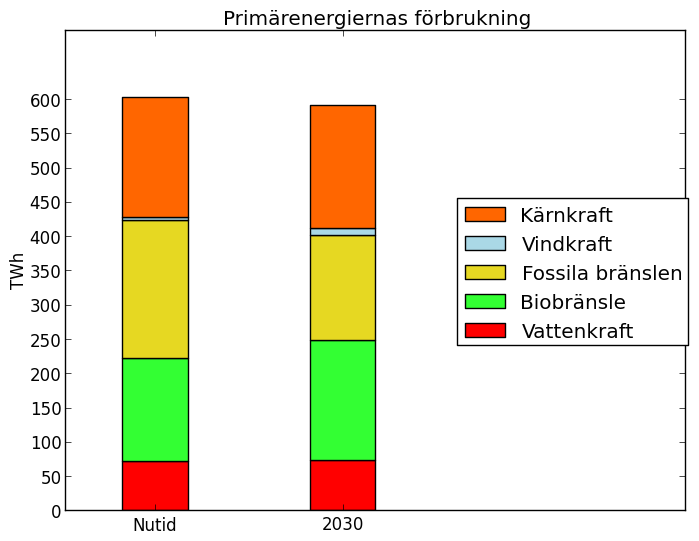
\includegraphics[scale=0.7]{scen1a1energidiagram.png}
       \caption{SKRIV NÅGOT HÄR}
       \label{fig:scen1a1energidiagram}
\end{figure}

Denna lösning stämmer ganska bra överens med den utveckling som regeringen förutspår i sin utredning. I de värden vi redovisat så har bilflottan varit nästintill helt fossil\textit{fri}, alltså en bit över gränsen till fossil\textit{oberoende}. Dock så finns stor möjlighet att falla tillbaka på fossila bränslen i de fall då det behövs. Detta kan vara till exempel då en oförutsägbar händelse radikalt förändrar landets energiförsörjning, såsom en ovanligt torr sommar som orsakar försämrad skörd av biomassa. Vi föreslår även att mer pengar satsas på forskning om el- och hybridfordonteknik, samt att styrmedel utnyttjas flitigt för att uppmuntra det Svenska folket att byta bil.

\subsubsection{Alternativ 2}

Idag används mycket biobränsle till uppvärmning. Om man istället börjar använda denna mängd till att tillverka drivmedel så kan det ersätta stora delar utav det fossila bränslet. Det kommer då behövas energier från andra källor för att ersätta biobränslet i andra sektorer. Detta skulle kunna ersättas med el. För att detta skall vara möjligt behöver Sveriges elproduktion öka till 2030. Sveriges riksdag har en planeringsram till år 2020 om att öka elproduktionen från 10 TWh till 30 TWh, en siffra som förmodligen kommer att vara ännu högre år 2030. Dessutom så räknas Sveriges reaktorer producera mer el 2030 än va de gör idag om inga reaktorer stängs ner.


\subsection{Scenario 2}
\begin{figure}[h!]
       \centering
       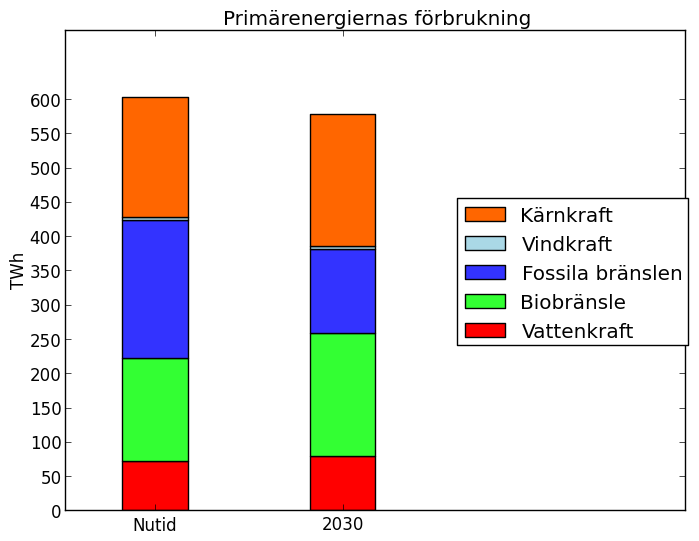
\includegraphics[scale=0.7]{scen2energidiagram.png}
       \caption{SKRIV NÅGOT HÄR}
       \label{fig:scen2energydiagram}
\end{figure}
I litteraturen så finns det inget om att vätgasbilar skulle ha någon större inverkan på bilflottan år 2030, dessutom så har finns det flera större rapporter där alla pekar på att antalet vätgasbilar kommer vara marginell.
Då utvecklingen utav vätgasbilar fortfarande är i ett stadie där det experimenteras mycket och modellerna endast finns i små mängder så har de ett väldigt högt inköpspris. För att vätgasbilar skall finnas i en större utbredning år 2030 så måste bilföretag välja att börja producera i större skalor så att priserna går ner.

Statliga medel som tvingar fram tankstationer är också ett måste då det för tillfället endast finns en tankstation i Malmö och två planerade, en vadera i Stockholm och Göteborg.

Ekonomiska medel från staten skulle göra att försäljningen kan öka tidigare då försäljningspriset kan vara högra utan att direkt påverka privatpersoners ekonomi.
Tyskland, Japan och Kalifornien är de platser där uppbyggnaden utav vätgasstationer har kommit längst. Där har myndigheter samarbetat med företag för att dela på kostnader och risker som det innebär. Sådana samarbeten skulle även behövas i Sverige om man snabba på uppbyggnaden av infrastruktur som stödjer vätgasbilar.
Detta är åtgärder som skulle behövas ta i kraft väldigt snart då Sverige för tillfäller inte har en nationell vätgas stratergi.

Något som talar för att utvecklingen för vätgasbilar skall gå framåt i snabbt takt är att det forskas på att använda vätgas som lagring för energi från exempelvis vindkraftverk. Detta skulle göra vindkraft mindre beroende av andra energikällor när det inte blåser. Utvecklingen av att binda energi i vätgas har alltså fördelar i andra områden än transport vilket gör att forskning inom området är lönsamt för flera. Det finns även industrier som har vätgas som spillvara som man kan ta vara på för att få vätgas direkt utan några energiförluster vid tillverkningen.

Hela detta scenariot är långt ifrån verkligheten. Bilar som drivs på vätgas med hjälp av bränsleceller ligger långt bakom bilar som drivs av el och biobränsle när det kommer till kommersiellt genomslag. Det krävs extrema årgärder för att det skall finnas en liten möjlighet till att det skall kunna genomföras och de åtgärderna måste ske snabbt. Dessutom skulle det innebära att all satsning på en ökad mängd elbilar och bilar som drivs på biobränsle behöver komma i andra hand. Detta är inte troligt då dessa förmodligen kommer få bort fossila bränslen från bilflottan och det finns ingen anledning till att minska den möjligheten. Bilar som drivs på vätgas har definitivt stor potential och kan komma att vara ett väldigt bra alternativ till fordon i framtiden, men det är fortfarande för tidigt. Till år 2030 lär vätgasbilar inte har någon stor inverkan.

\subsection{Slutsats}
Det är möjligt att göra Sveriges bilflotta fossilfri, men det kommer att behövas åtgärder; både ekonomiska och struktuella. Vissa åtgärder är redan tagna och andra är på gång. Att bilflottan blir fossilfri bidrar inte bara till klimatmålen utan bidrar även till attraktivare städer, långsiktigt lägre kostnader, attraktivare städer och förbättrad hälsa. Denna kombination gör det högst troligt att nuvarande regering och kommande regeringar kommer driva igenom de styrmedel som krävs. Lösningen lär ligga i elbilar och bilar som drivs på biobränsle, det är de fordon som kommit längst i utvecklingen och de Sveriges infrastruktur har stöd för och en plan för när det kommer till miljövänliga fordon. Det är oklart hur man kommer gå till väga, både med styrmedel och ändrad energifördelning. Det finns flera möjliga lösningar, fler än de vi gått igenom, och det är svårt att veta hur det kommer se ut i framtiden. En sak som är säkert kommande åren är kritiska för att lyckas nå målen och det är en stor utmaning.
\printbibliography
\end{document}

